\chapter{Практическая Часть}
В данной части представлен листинг и результат работы программы.
\section{Листиниг программы}
\begin{lstlisting}
function lab1()
X = [11.89,9.60,9.29,10.06,9.50,8.93,9.58,6.81,8.69,9.62,
9.01,10.59,10.50,11.53,9.94,8.84,8.91,6.90,9.76,7.09,11.29,
11.25,10.84,10.76,7.42,8.49,10.10,8.79,11.87,8.77,9.43,12.41,
9.75,8.53,9.72,9.45,7.20,9.23,8.93,9.15,10.19,9.57,11.09,9.97,
8.81,10.73,9.57,8.53,9.21,10.08,9.10,11.03,10.10,9.47,9.72,9.60,
8.21,7.78,10.21,8.99,9.14,8.60,9.14,10.95,9.33,9.98,9.09,10.35,
8.61,9.35,10.04,7.85,9.64,9.99,9.65,10.89,9.08,8.60,7.56,9.27,
10.33,10.09,8.51,9.86,9.24,9.63,8.67,8.85,11.57,9.85,9.27,9.69,
10.90,8.84,11.10,8.19,9.26,9.93,10.15,8.42,9.36,9.93,9.11,9.07,
7.21,8.22,9.08,8.88,8.71,9.93,12.04,10.41,10.80,7.17,9.00,9.46,
10.42,10.43,8.38,9.01];
X = sort(X);
Mmax = max(X);
Mmin = min(X);
fprintf('Mmin = %s\n', num2str(Mmin));
fprintf('Mmax = %s\n', num2str(Mmax));
R = Mmax - Mmin;
fprintf('R = %s\n', num2str(R));
MU = getMU(X);
fprintf('MU = %s\n', num2str(MU));
Ssqr = getSsqr(X);
fprintf('S^2 = %s\n', num2str(Ssqr));
m = getNumberOfIntervals(X);
fprintf('m = %s\n', num2str(m))
createGroup(X);
hold on;
distributionDensity(X, MU, Ssqr, m);
figure;
empiricF(X);
hold on;
distribution(X, MU, Ssqr, m);
end
\end{lstlisting}
\newpage
\begin{lstlisting}
function mu = getMU(X)
n = length(X);
mu = sum(X)/n;
end
function Ssqr = getSsqr(X)
n = length(X);
MX = getMU(X);
Ssqr = sum((X - MX).^2) / (n-1);
end
function m = getNumberOfIntervals(X)
m = floor(log2(length(X)) + 2);
end
function createGroup(X)
n = length(X);
m = getNumberOfIntervals(X);
intervals = zeros(1, m+1);
numCount = zeros(1, m+1);
Delta = (max(X) - min(X)) / m;
for i = 0: m
intervals(i+1) = X(1) + Delta * i;
end
j = 1;
count = 0;
for i = 1:n
if (X(i) >= intervals(j+1))
j = j + 1;
end
numCount(j) = numCount(j) + 1;
count = count + 1;
end
graphBuf = numCount(1:m+1);
for i = 1:m+1
graphBuf(i) = numCount(i) / (n*Delta);
end
stairs(intervals, graphBuf),grid;
end
\end{lstlisting}
\newpage
\begin{lstlisting}
function distributionDensity(X, MX, DX, m)
R = X(end) - X(1);
delta = R/m;
Sigma = sqrt(DX);
Xn = (MX - R): delta/50 :(MX + R);
Y = normpdf(Xn, MX, Sigma);
plot(Xn, Y), grid;
end
function distribution(X, MX, DX, m)
R = X(end) - X(1);
delta = R/m;
Xn = (MX - R): delta :(MX + R);
Y = 1/2 * (1 + erf((Xn - MX) / sqrt(2*DX)));
plot(Xn, Y, 'r'), grid;
end
function empiricF(X)
[yy, xx] = ecdf(X);
stairs(xx, yy), grid;
end
\end{lstlisting}

\section{Результат работы программы}
\begin{equation*}
    \begin{split}
        &M_{min} = 6.81\\
        &M_{max} = 12.41\\
        &R = 5.6\\
        &\hat{\mu}(\Vec{X_n}) = 9.4872\\
        &S^2(\Vec{X_n}) = 1.2173\\
        &m = 8
    \end{split}
\end{equation*}
\newpage

\section{Графики}

\begin{figure}[h!]
    \centering
    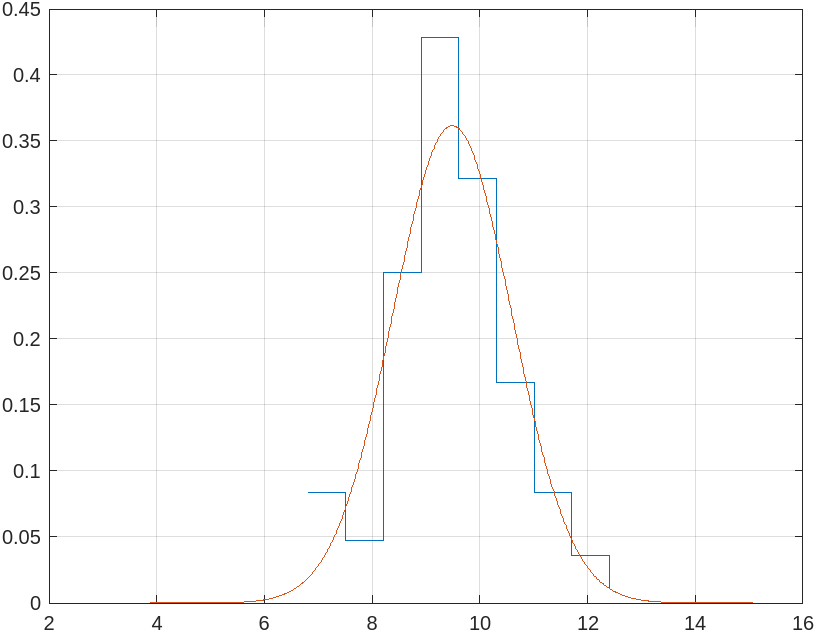
\includegraphics[]{images/first_number.png}
    \caption{Гистограмма и график функции плотности распределения
нормальной случайной величины.}
\end{figure}

\begin{figure}[h!]
    \centering
    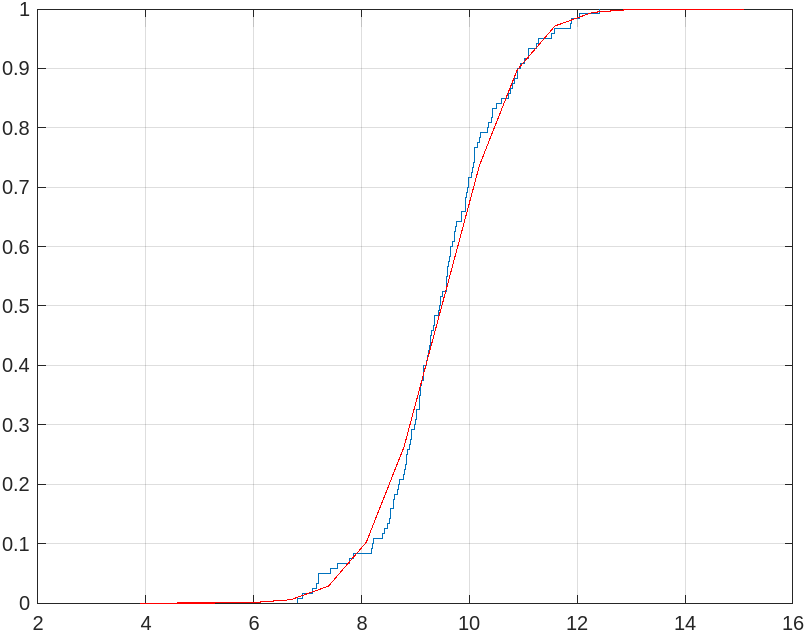
\includegraphics[]{images/second_number.png}
    \caption{График эмпирической функции распределения и функции
распределения нормальной случайной величины}
\end{figure}
